\chapter{การทดสอบวัดประสิทธิภาพ และผลการทดลอง}

\section{การทดสอบประสิทธิภาพของ ML Kit}

\subsection{วัตถุประสงค์}
เพื่อทดสอบประสิทธิภาพการทำงานของ ML Kit ในการตรวจจับท่าทางในสภาวะแวดล้อมที่แตกต่างกันว่าสามารถตรวจจับจุดต่าง ๆ ตามร่างกายได้ครบทั้ง 33 จุด (Landmarks) หรือไม่

\subsection{วิธีการทดลอง}
\begin{enumerate}
	\item ตั้งกล้องหน้าโทรศัพท์มือถือในสภาวะที่มีแสงสว่างเพียงพอ
	\item จับภาพจากกล้องหน้าโทรศัพท์มือถือ
	\item ทดสอบการยืนหน้ากล้อง โดยให้กล้องเห็นรูปร่างทั้งตัว
	\item นำภาพที่ได้ผ่านกระบวนการตรวจจับความเคลื่อนไหว (Pose Detection)
	\item ML Kit จะทำการส่งค่าเป็นพิกัดตามจุดต่าง ๆ ของร่างกาย ซึ่งจะได้พิกัดแกน X, Y, Z, และ likelihood ซึ่ง likelihood จะเป็นค่าช่วงความเชื่อมั่นที่จุด Landmark นั้น ๆ สามารถตรวจจับได้ ซึ่งในการทดสอบนี้จะใช้ช่วงความเชื่อมั่นที่มากกว่า 90\% ในการทดสอบประสิทธิภาพ
	\item ทำการสุ่มผลลัพธ์ที่ได้จากข้อ 5 มา 5 เฟรม เพื่อเก็บค่า likelihood ของพิกัดจุดร่างกายทั้ง 33 จุด
	\item ทำการเปลี่ยนสภาพแวดล้อมให้กล้องหน้าโทรศัพท์มือถือให้อยู่ในสภาวะที่แสงน้อย, มีวัตถุอื่น ๆ มารบกวนในภาพ, สีเสื้อที่กลมกลืนกับร่างกาย, มีบุคคลที่อยู่ด้านหลังฉาก จากนั้นดำเนินการข้อ 2 – 6 อีกครั้ง
	\item ทำการวิเคราะห์ค่า likelihood ที่ได้ว่ามีช่วงความเชื่อมั่นที่มากกว่า 90\% หรือไม่
\end{enumerate}

\subsection{ผลการทดลอง}
จากการทดลองประสิทธิภาพการทำงานของ ML Kit ในการตรวจจับท่าทาง โดยได้ทำการทดสอบในสภาวะแวดล้อมที่แตกต่างกันทั้ง 5 สภาวะ ได้แก่สภาวะที่มีแสงสว่างเพียงพอ, สภาวะที่มีแสงน้อย, สภาวะที่มีวัตถุอื่น ๆ มารบกวนในภาพ, สภาวะที่สีเสื้อที่กลมกลืนกับร่างกาย, และสภาวะที่มีบุคคลอื่นอยู่ด้านหลังฉากนั้นได้ผลลัพธ์ดังนี้
\subsubsection{การตั้งกล้องหน้าโทรศัพท์มือถือในสภาวะที่มีแสงสว่างเพียงพอ}
ค่า likelihood ที่ได้รับจาก ML Kit นั้นมีค่าความเชื่อมั่นในจุดต่าง ๆ บนร่างกายทั้ง 33 จุดที่มากกว่า 95\% ทั้ง 5 เฟรม
\begin{figure}
	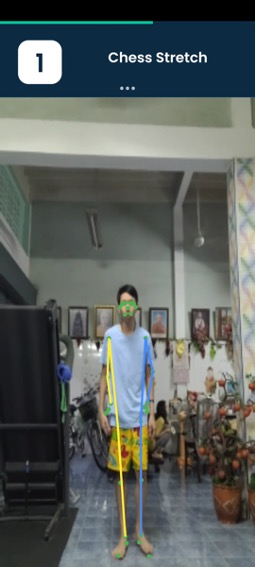
\includegraphics[width=4cm]{./chapter_4/4-1.jpg}
	\caption{การตรวจจับท่าทางในสภาวะที่มีแสงสว่างเพียงพอ}
\end{figure}
\begin{figure}
	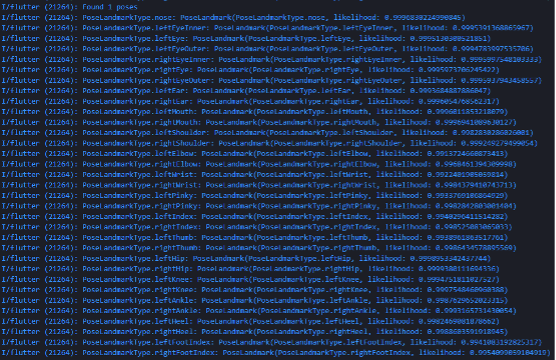
\includegraphics[width=15cm]{./chapter_4/4-2.png}
	\caption{ตัวอย่างผลลัพธ์ที่ได้ในสภาวะที่มีแสงสว่างเพียงพอ}
\end{figure}
\subsubsection{การตั้งกล้องหน้าโทรศัพท์มือถือในสภาวะที่มีแสงน้อย}
ค่า likelihood ที่ได้รับจาก ML Kit นั้นมีค่าความเชื่อมั่นในจุดต่าง ๆ บนร่างกายทั้ง 33 จุดที่มากกว่า 95\% ทั้ง 5 เฟรม
\begin{figure}
	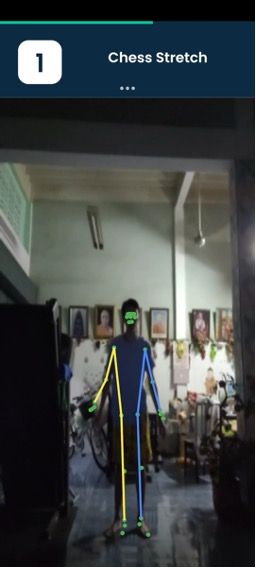
\includegraphics[width=4cm]{./chapter_4/4-3.jpg}
	\caption{การตรวจจับท่าทางในสภาวะที่มีแสงน้อย}
\end{figure}
\begin{figure}
	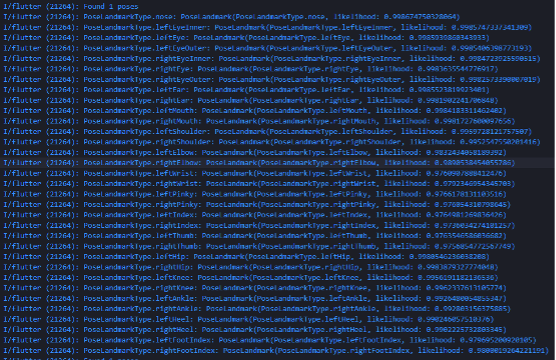
\includegraphics[width=15cm]{./chapter_4/4-4.png}
	\caption{ตัวอย่างผลลัพธ์ที่ได้ในสภาวะที่มีแสงน้อย}
\end{figure}
\subsubsection{การตั้งกล้องหน้าโทรศัพท์มือถือในสภาวะที่มีวัตถุอื่น ๆ มารบกวนในภาพ}
ค่า likelihood ที่ได้รับจาก ML Kit นั้นมีค่าความเชื่อมั่นในจุดต่าง ๆ บนร่างกายทั้ง 33 จุดที่มากกว่า 95\% ทั้ง 5 เฟรม
\begin{figure}
	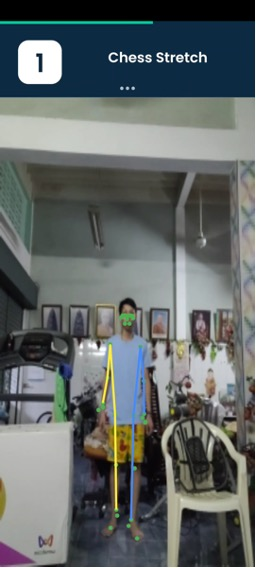
\includegraphics[width=4cm]{./chapter_4/4-5.jpg}
	\caption{การตรวจจับท่าทางในสภาวะที่มีวัตถุอื่น ๆ มารบกวนในภาพ}
\end{figure}
\begin{figure}
	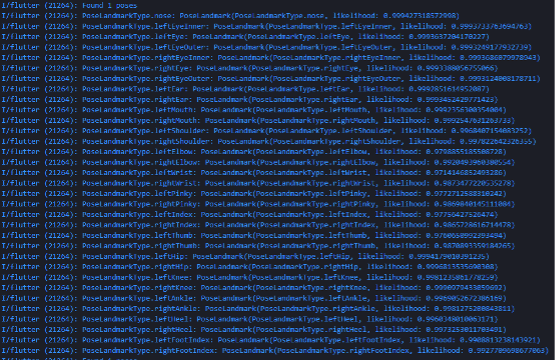
\includegraphics[width=15cm]{./chapter_4/4-6.png}
	\caption{ตัวอย่างผลลัพธ์ที่ได้ในสภาวะที่มีวัตถุอื่น ๆ มารบกวนในภาพ}
\end{figure}
\subsubsection{การตั้งกล้องหน้าโทรศัพท์มือถือในสภาวะที่สีเสื้อที่กลมกลืนกับร่างกาย}
ค่า likelihood ที่ได้รับจาก ML Kit นั้นมีค่าความเชื่อมั่นในจุดต่าง ๆ บนร่างกายทั้ง 33 จุดที่มากกว่า 95\% ทั้ง 5 เฟรม
\begin{figure}
	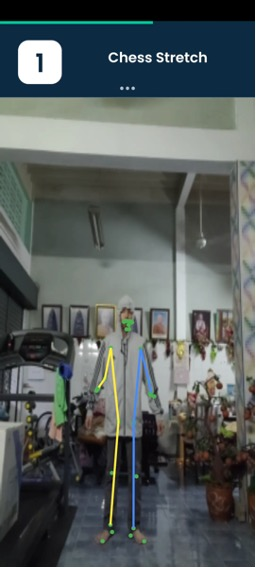
\includegraphics[width=4cm]{./chapter_4/4-7.jpg}
	\caption{การตรวจจับท่าทางในสภาวะที่สีเสื้อที่กลมกลืนกับร่างกาย}
\end{figure}
\begin{figure}
	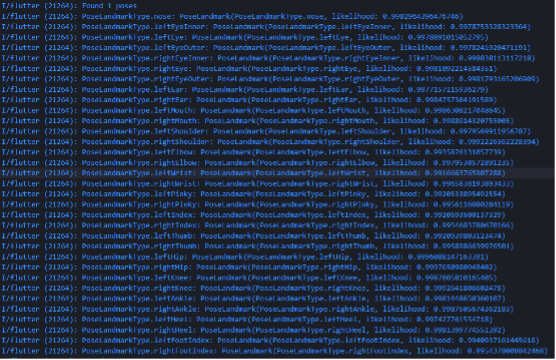
\includegraphics[width=15cm]{./chapter_4/4-8.png}
	\caption{ตัวอย่างผลลัพธ์ที่ได้ในสภาวะที่สีเสื้อที่กลมกลืนกับร่างกาย}
\end{figure}
\subsubsection{การตั้งกล้องหน้าโทรศัพท์มือถือในสภาวะที่มีบุคคลอื่นอยู่ด้านหลังฉาก}
ในการตรวจจับท่าทางในกรณีที่มีบุคคลอื่นอยู่ด้านหลังฉากนั้น เมื่อเริ่มต้นระบบจะทำการตรวจจับท่าทาง และเมื่อพบร่างกายแล้วระบบจะทำการกำหนดค่า Landmarks ทั้ง 33 จุดให้กับบุคคลที่มีค่า likelihood หรือช่วงความเชื่อมั่นที่สูงที่สุด จากรูปที่ 4.9 นั้น ระบบได้ตรวจพบเพียงบุคคลเดียว จากนั้นเมื่อมีบุคคลอื่นที่เข้ามาอยู่ในเฟรม ระบบยังคงกำหนดค่า Landmarks ให้กับบุคคลเดิม ไม่ว่าบุคคลอื่นจะอยู่ในระยะของกล้องเท่าใดก็ตาม เนื่องจากบุคคลเดิมนั้นยังมีค่าช่วงความเชื่อมั่นที่สูงกว่าบุคคลอื่น ตามรูปที่ 4.10, 4.11, 4.12 โดยค่าที่ได้รับจาก ML Kit นั้นมีค่าความเชื่อมั่นในจุดต่าง ๆ บนร่างกายทั้ง 33 จุดที่มากกว่า 95\% ทั้ง 5 เฟรม
\begin{figure}
	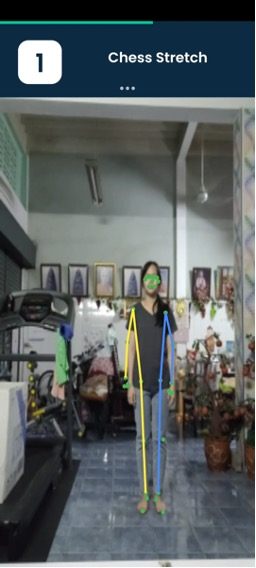
\includegraphics[width=4cm]{./chapter_4/4-9.jpg}
	\caption{การตรวจจับท่าทางในสภาวะที่มีบุคคลอื่นอยู่ด้านหลังฉาก}
\end{figure}
\begin{figure}
	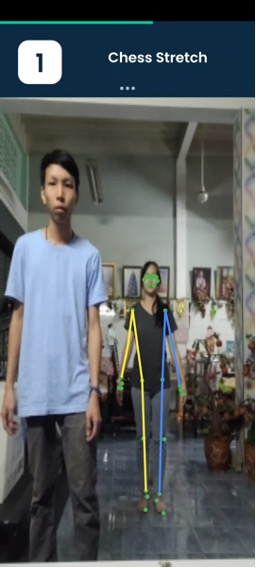
\includegraphics[width=4cm]{./chapter_4/4-10.jpg}
	\caption{การตรวจจับท่าทางในสภาวะที่มีบุคคลอื่นอยู่ด้านหลังฉาก}
\end{figure}
\begin{figure}
	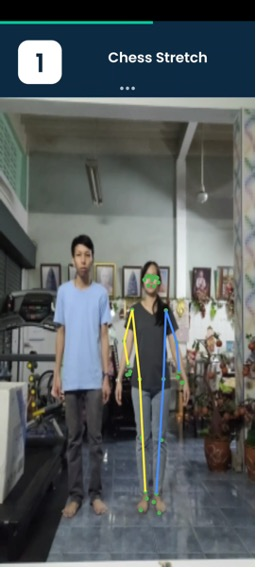
\includegraphics[width=4cm]{./chapter_4/4-11.jpg}
	\caption{การตรวจจับท่าทางในสภาวะที่มีบุคคลอื่นอยู่ด้านหลังฉาก}
\end{figure}
\begin{figure}
	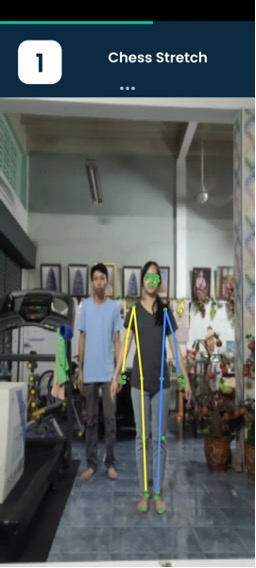
\includegraphics[width=4cm]{./chapter_4/4-12.jpg}
	\caption{การตรวจจับท่าทางในสภาวะที่มีบุคคลอื่นอยู่ด้านหลังฉาก}
\end{figure}
\begin{figure}
	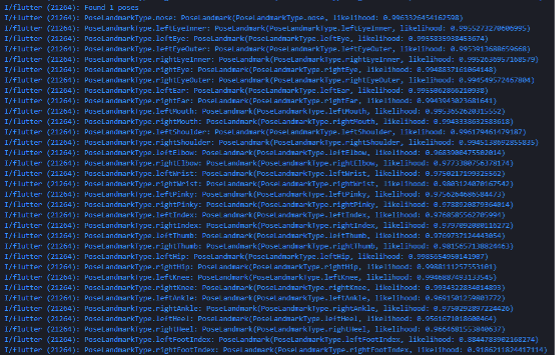
\includegraphics[width=15cm]{./chapter_4/4-13.png}
	\caption{ตัวอย่างผลลัพธ์ที่ได้ในสภาวะที่มีบุคคลอื่นอยู่ด้านหลังฉาก}
\end{figure}

\section{การทดสอบวัดประสิทธิภาพของฟังก์ชันการคำนวณองศา}
\subsection{วัตถุประสงค์}
เพื่อทดสอบประสิทธิภาพของฟังก์ชันการคำนวณองศา หลังจากให้ ML Kit ตรวจสอบท่าทางและได้ส่งค่าพิกัดจุดต่าง ๆ บนร่างกายกลับมา ว่าสามารถวัดองศาของของจุดข้อต่อของร่างกายได้หรือไม่
\subsection{วิธีการทดลอง}
\begin{enumerate}
	\item จับภาพจากกล้องหน้าโทรศัพท์มือถือ
	\item ทดสอบการยืนหน้ากล้อง โดยให้กล้องเห็นรูปร่างทั้งตัว และออกท่าทางต่าง ๆ ในการทดสอบองศา ได้แก่ท่าทางยืนตรง, กางแขนซ้าย, และยกมือซ้าย
	\item นำภาพที่ได้ผ่านกระบวนการตรวจจับความเคลื่อนไหว (Pose Detection) ของ ML Kit
	\item เมื่อได้ผลลัพธ์เป็นพิกัดจุดต่าง ๆ ของร่างกายจากข้อ 3 แล้วจึงนำค่าดังกล่าวเข้าสู่ฟังก์ชันการคำนวณองศาที่ได้พัฒนาขึ้น และได้กำหนดค่าในการหาองศาของข้อศอกซ้าย(Left Elbow) และสะโพกซ้าย (Left Hip) ที่ทำมุมกับหัวไหล่ซ้าย (Left Shoulder)
	\item ทำการนำผลลัพธ์ที่ได้จากข้อ 4 มา 5 เฟรม เพื่อเก็บค่าองศาของพิกัดจุดร่างกาย
	\item ทำการวิเคราะห์ค่าองศาที่ได้จากฟังก์ชันดังกล่าวว่ามีค่าความคลาดเคลื่อนจากองศาในอุดมคติไม่เกิน 5\% หรือไม่ โดยใช้สมการหาความคลาดเคลื่อนจาก
	      \begin{equation}
		      Tolerance_\%=\frac{degree_{measure} - degree_{ideal}}{360} \times 100
	      \end{equation}
\end{enumerate}
\subsection{ผลการทดลอง}
จากการทดลองประสิทธิภาพของฟังก์ชันการคำนวณองศาของการออกท่าทางทั้ง 3 ท่าทาง ได้แก่ท่าทางยืนตรง, ท่าทางกางแขนซ้าย, และท่าทางยกมือซ้ายนั้นได้ผลลัพธ์ดังนี้
\subsubsection{ท่าทางยืนตรง}
การวัดองศาของข้อศอกซ้ายและสะโพกซ้าย ที่ทำมุมกับหัวไหล่ซ้าย ในท่าทางยืนตรงนั้น มีค่าองศาในอุดมคติคือ 0 องศา จากการนำค่าองศาที่ได้จากฟังก์ชันการคำนวณองศาทั้ง 5 เฟรมนั้น ซึ่งมีค่าที่ได้ ได้แก่ 10.44, 9.04, 6.04, 10.77, และ 9.39 องศาตามลำดับ ซึ่งค่าองศาดังกล่าวมีค่าความคลาดเคลื่อนจากองศาในอุดมคติไม่เกิน 5\%
\begin{figure}
	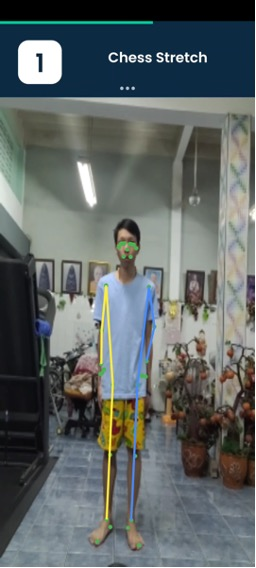
\includegraphics[width=4cm]{./chapter_4/4-14.jpg}
	\caption{การตรวจจับท่าทางในท่ายืนตรง}
\end{figure}
\begin{figure}
	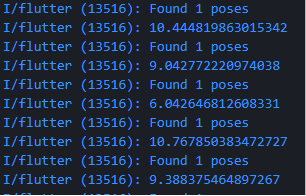
\includegraphics[width=7cm]{./chapter_4/4-15.png}
	\caption{ตัวอย่างผลลัพธ์ที่ได้ในท่าทางยืนตรง}
\end{figure}
\subsubsection{ท่าทางกางแขนซ้าย}
การวัดองศาของข้อศอกซ้ายและสะโพกซ้าย ที่ทำมุมกับหัวไหล่ซ้าย ในท่าทางกางแขนซ้ายนั้น มีค่าองศาในอุดมคติคือ 90 องศา จากการนำค่าองศาที่ได้จากฟังก์ชันการคำนวณองศาทั้ง 5 เฟรมนั้น ซึ่งมีค่าที่ได้ ได้แก่ 99.25, 99.88, 98.06, 93.48, และ 90.39 องศาตามลำดับ ซึ่งค่าองศาดังกล่าวมีค่าความคลาดเคลื่อนจากองศาในอุดมคติไม่เกิน 5\%
\begin{figure}
	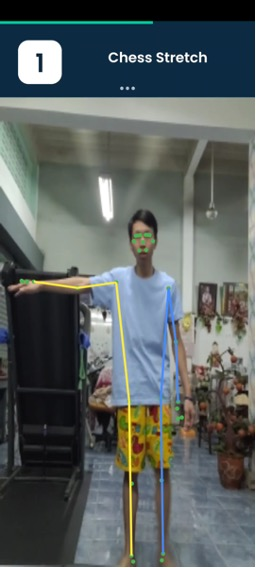
\includegraphics[width=4cm]{./chapter_4/4-16.jpg}
	\caption{การตรวจจับท่าทางในท่ากางแขนซ้าย}
\end{figure}
\begin{figure}
	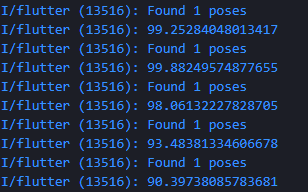
\includegraphics[width=7cm]{./chapter_4/4-17.png}
	\caption{ตัวอย่างผลลัพธ์ที่ได้ในท่าทางกางแขนซ้าย}
\end{figure}
\subsubsection{ท่าทางยกมือซ้าย}
การวัดองศาของข้อศอกซ้ายและสะโพกซ้าย ที่ทำมุมกับหัวไหล่ซ้าย ในท่าทางยืนตรงนั้น มีค่าองศาในอุดมคติคือ 0 องศา จากการนำค่าองศาที่ได้จากฟังก์ชันการคำนวณองศาทั้ง 5 เฟรมนั้น ซึ่งมีค่าที่ได้ ได้แก่ 173.20, 170.41, 174.56, 173.44, และ 172.92 องศา ซึ่งค่าองศาดังกล่าวมีค่าความคลาดเคลื่อนจากองศาในอุดมคติไม่เกิน 5\%
\begin{figure}
	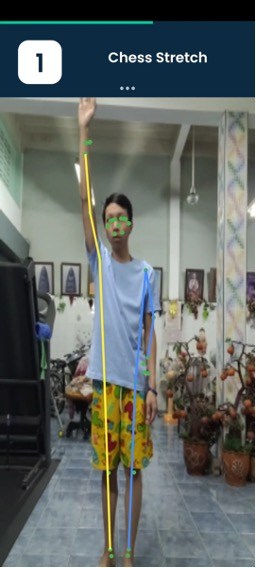
\includegraphics[width=4cm]{./chapter_4/4-18.jpg}
	\caption{การตรวจจับท่าทางในท่ายกมือซ้าย}
\end{figure}
\begin{figure}
	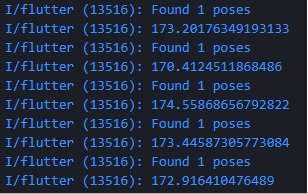
\includegraphics[width=7cm]{./chapter_4/4-19.png}
	\caption{ตัวอย่างผลลัพธ์ที่ได้ในท่าทางยกมือซ้าย}
\end{figure}

\section{การทดสอบวัดประสิทธิภาพความแม่นยำในการตรวจจับของ ML Kit}
\subsection{วัตถุประสงค์}
การทดลองนี้มีวัตถุประสงค์เพื่อทดสอบประสิทธิภาพความแม่นยำในการตรวจจับของ ML Kit ว่าสามารถทำงานได้ตามที่คาดหวังหรือไม่
\subsection{วิธีการทดลอง}
\begin{enumerate}
	\item จับภาพจากกล้องหน้าโทรศัพท์มือถือ
	\item ทดสอบโดยการยืนหน้ากล้อง โดยให้กล้องเห็นรูปร่างทั้งตัว และออกท่าการออกกำลังกาย ได้แก่ท่าทางกระโดดตบ, ลุกนั่ง (Squats) เป็นจำนวนท่าทางละ 10 ครั้ง
	\item นำภาพที่ได้ผ่านกระบวนการตรวจจับความเคลื่อนไหว (Pose Detection) ของ ML Kit
	\item เมื่อได้ผลลัพธ์เป็นพิกัดจุดต่าง ๆ ของร่างกายจากข้อ 3 แล้วจึงนำค่าดังกล่าวเข้าสู่อัลกอริทึมการตรวจสอบท่าทางของผู้ใช้ โดยได้นำไฟล์ข้อมูลท่าทางการออกกำลังกายเข้ามาตรวจสอบร่วมด้วย
	\item ระหว่างการทำการออกท่าทางดังกล่าว มีการบันทึกค่า \% likelihood ทุก ๆ 500 มิลลิวินาที
	\item เมื่อทำการออกท่าการออกกำลังกายครบจำนวน 10 ครั้งแล้ว จีงตรวจสอบและบันทึกผลจำนวนครั้งที่การตรวจจับของ ML Kit สามารถนับได้
	\item ทำการบันทึกผล \% likelihood เฉลี่ยของ Landmark ร่างกายต่าง ๆ
	\item ทำการทดสอบในข้อ 2 - 7 อีกครั้งหนึ่ง โดยเปลี่ยนจากการยืนหน้ากล้อง เป็นการใช้วิดีโอสาธิตท่าทางการออกกำลังกายต้นฉบับ
	\item ทำการวิเคราะห์และเปรียบเทียบจำนวนครั้งที่ได้ และ \% likelihood เฉลี่ยจากการตรวจจับดังกล่าว ทั้งจากการยืนหน้ากล้องและใช้วิดีโอสาธิตการออกกำลังกายต้นฉบับว่าสามารถทำงานได้ตามที่คาดหวังหรือไม่
\end{enumerate}
\subsection{ผลการทดลอง}
จากการทดลองประสิทธิภาพความแม่นยำในการตรวจจับของ ML Kit ของการออกท่าทางการออกกำลังกายทั้ง 4 ท่าทาง ได้แก่ท่าทางกระโดดตบ, ลุกนั่ง (Squats) เป็นจำนวนท่าทางละ 10 ครั้งนั้นได้ผลลัพธ์ดังนี้
\subsubsection{ท่าทางกระโดดตบ}
การนับจำนวนครั้งที่ได้จากการตรวจจับของ ML Kit ในท่าทางกระโดดตบนั้นสามารถนับได้ 10 ครั้ง ทั้งจากการยืนหน้ากล้องและใช้วิดีโอสาธิตการออกกำลังกายต้นฉบับ โดย \% likelihood เฉลี่ยของ Landmark ของการออกท่าทางทั้งสองรูปแบบเป็นดังนี้
\begin{table}
	\centering
	\caption{รายละเอียดความแม่นยำในการตรวจจับของ ML Kit ของท่าทางกระโดดตบ}
	\begin{tabularx}{\linewidth}{ | >{\centering}X| >{\centering}X|X|X|X|X|X|X|}
		\hline
		\multirow{2}{*}{ท่าทาง} & \multirow{2}{*}{\shortstack{จำนวน\\ครั้ง}} & \multicolumn{6}{c|}{\% likelihood (Average)}                                                                   \\
		\cline{3-8}
		                       &                          & right Elbow                                  & rightHip & right Shoulder & leftElbow & leftHip & left Shoulder \\
		\hline
		กระโดดตบ               & 10                       & 71.16\%                                      & 86.52\%  & 79.75\%        & 90.34\%   & 91.09\% & 98.90\%       \\
		\hline
		กระโดดตบ (ต้นฉบับ)       & 10                       & 99.29\%                                      & 99.97\%  & 99.80\%        & 99.00\%   & 99.90\% & 99.80\%       \\
		\hline
	\end{tabularx}
\end{table}
\subsubsection{ท่าทางลุกนั่ง (Squats)}
การนับจำนวนครั้งที่ได้จากการตรวจจับของ ML Kit ในท่าทางลุกนั่งนั้นสามารถนับได้ 10 ครั้ง ทั้งจากการยืนหน้ากล้องและใช้วิดีโอสาธิตการออกกำลังกายต้นฉบับ โดย \% likelihood เฉลี่ยของ Landmark ของการออกท่าทางทั้งสองรูปแบบเป็นดังนี้
\begin{table}
	\centering
	\caption{รายละเอียดความแม่นยำในการตรวจจับของ ML Kit ของท่าทางลุกนั่ง (Squats)}
	\begin{tabularx}{\linewidth}{| >{\centering}X| >{\centering}X|X|X|X|X|X|X|}
		\hline
		\multirow{2}{*}{ท่าทาง} & \multirow{2}{*}{\shortstack{จำนวน\\ครั้ง}} & \multicolumn{6}{c|}{\% likelihood (Average)}                                                                       \\
		\cline{3-8}
		                       &                          & right Elbow                                  & rightWrist & right Shoulder & leftElbow & leftWrist & left Shoulder \\
		\hline
		Squats                 & 10                       & 99.26\%                                      & 99.76\%    & 99.92\%        & 99.74\%   & 99.36\%   & 99.97\%       \\
		\hline
		Squats ~(ต้นฉบับ)        & 10                       & 92.83\%                                      & 93.60\%    & 97.88\%        & 94.30\%   & 93.77\%   & 99.91\%       \\
		\hline
	\end{tabularx}
\end{table}
\begin{table}
	\centering
	\caption{รายละเอียดความแม่นยำในการตรวจจับของ ML Kit ของท่าทางลุกนั่ง (Squats) ต่อ}
	\begin{tabularx}{\linewidth}{| >{\centering}X| >{\centering}X|X|X|X|X|X|X|}
		\hline
		\multirow{2}{*}{ท่าทาง} & \multirow{2}{*}{\shortstack{จำนวน\\ครั้ง}} & \multicolumn{6}{c|}{\% likelihood (Average)}                                                            \\
		\cline{3-8}
		                       &                          & rightHip                                     & right Ankle & rightKnee & leftHip & leftAnkle & leftKnee \\
		\hline
		Squats                 & 10                       & 99.97\%                                      & 95.61\%     & 99.37\%   & 99.98\% & 95.19\%   & 98.91\%  \\
		\hline
		Squats ~(ต้นฉบับ)        & 10                       & 92.92\%                                      & 90.75\%     & 92.24\%   & 93.08\% & 90.47\%   & 91.83\%  \\
		\hline
	\end{tabularx}
\end{table}

\section{การทดสอบส่วนการติดต่อผู้ใช้ (User Interface)}
\subsection{วัตถุประสงค์}
เพื่อทดสอบการทำงานของส่วนการติดต่อผู้ใช้ (User Interface) ว่าสามารถทำงานได้ตามที่คาดหวังหรือไม่
\subsection{วิธีการทดลอง}
ทดลองการใช้งานการกดปุ่มทุกปุ่มที่มีในแอปพลิเคชันว่าสามารถทำงานได้ และนำทางไปยังหน้าที่คาดหวังได้
\subsection{ผลการทดลอง}
จากการทดสอบการทำงานของส่วนการติดต่อผู้ใช้ดังกล่าวพบว่าปุ่มทุกปุ่มสามารถทำงาน และนำทางได้ตามที่คาดหวัง
\begin{figure}
	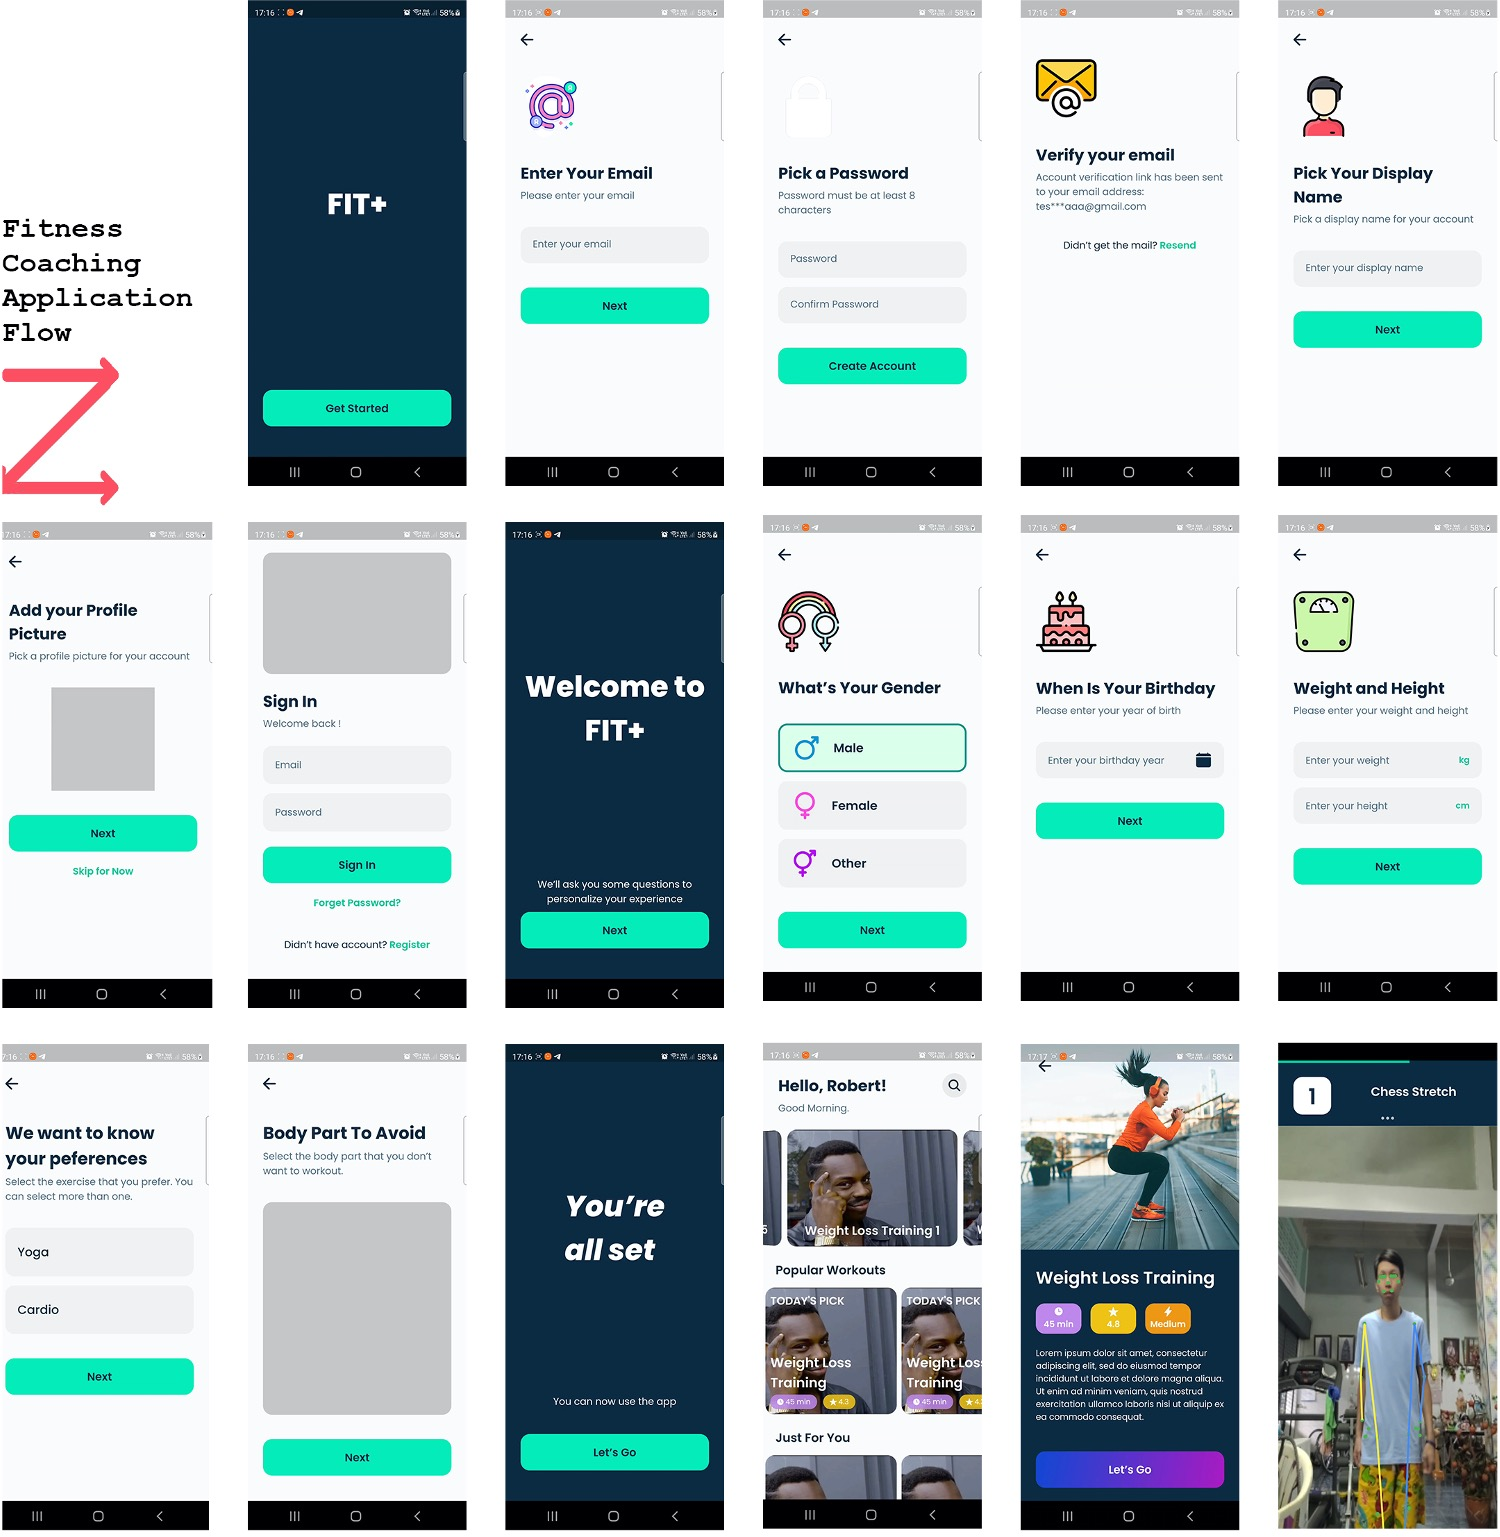
\includegraphics[width=15cm]{./chapter_4/4-20.jpg}
	\caption{ตัวอย่างการทำงานของหน้าจอผู้ใช้ในแอปพลิเคชัน}
\end{figure}

\section{การทดสอบระบบ API}
\subsection{วัตถุประสงค์}
การทดลองนี้มีวัตถุประสงค์เพื่อทดสอบการทำงานของ API ว่ามีการทำงานที่ถูกต้องเป็นไปตามที่ได้ออกแบบไว้ โดยจะทดสอบ API ที่ได้ Deploy ไปบน Google Cloud Functions
\subsection{วิธีการทดลอง}
\begin{enumerate}
	\item ใช้โปรแกรม Postman ในการทดสอบ
	\item พิมพ์ URL ของ API ที่ต้องการทดสอบ รวมถึง parameter และ token ต่าง ๆ ที่จำเป็น
	\item กด Send เพื่อส่งข้อมูลไปยัง API
	\item รอการตอบกลับจาก API แล้วจึงบันทึกผลที่ได้
\end{enumerate}
\subsubsection{ผลการทดลอง}
\begin{figure}
	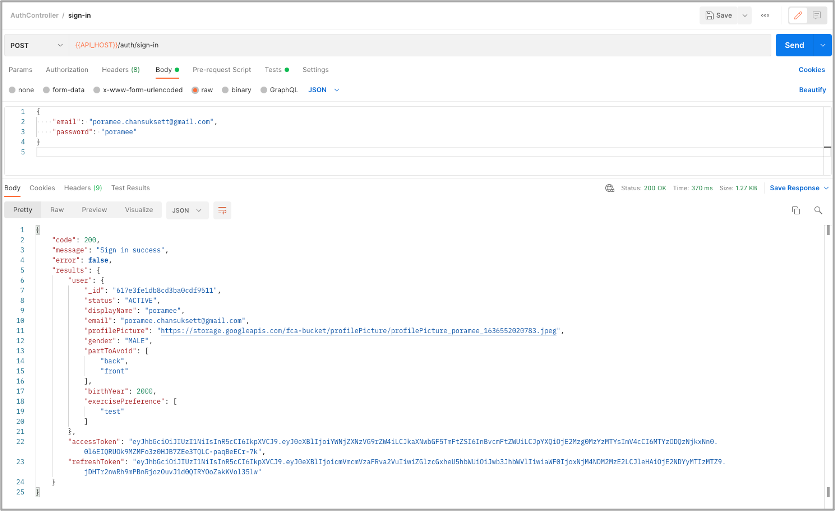
\includegraphics[width=15cm]{./chapter_4/API-signin.png}
	\caption{แสดงผลการทดลอง API ของการเข้าสู่ระบบ แบบกรอกข้อมูลถูกต้อง}
\end{figure}
\begin{figure}
	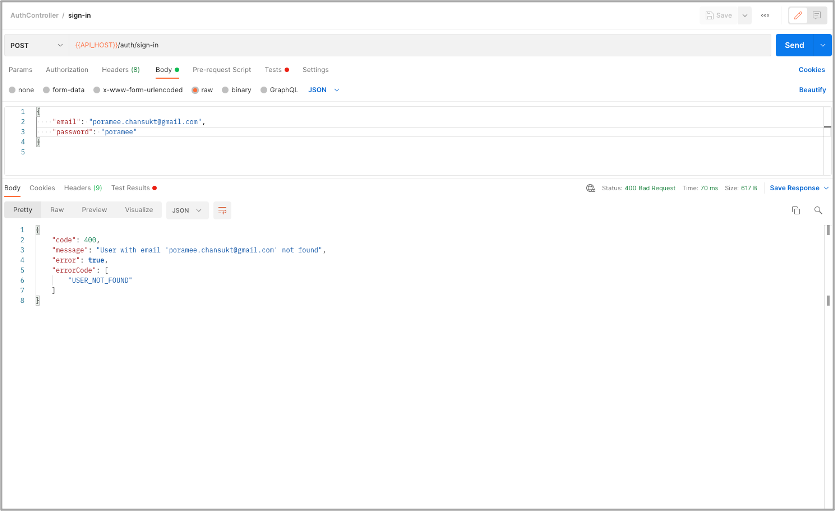
\includegraphics[width=15cm]{./chapter_4/API-signin-incorrect.png}
	\caption{แสดงผลการทดลอง API ของการเข้าสู่ระบบ แบบกรอกอีเมลไม่ถูกต้อง}
\end{figure}
\begin{figure}
	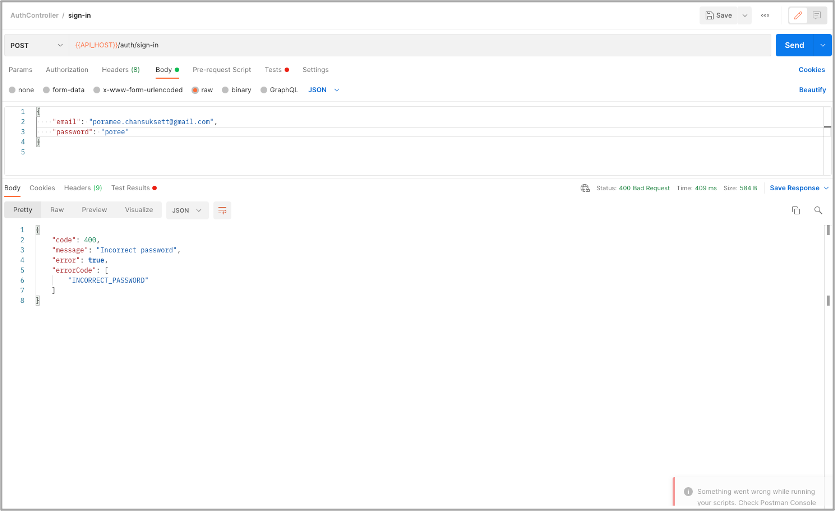
\includegraphics[width=15cm]{./chapter_4/API-signin-incorrect2.png}
	\caption{แสดงผลการทดลอง API ของการเข้าสู่ระบบ แบบกรอกรหัสผ่านไม่ถูกต้อง}
\end{figure}
\begin{figure}
	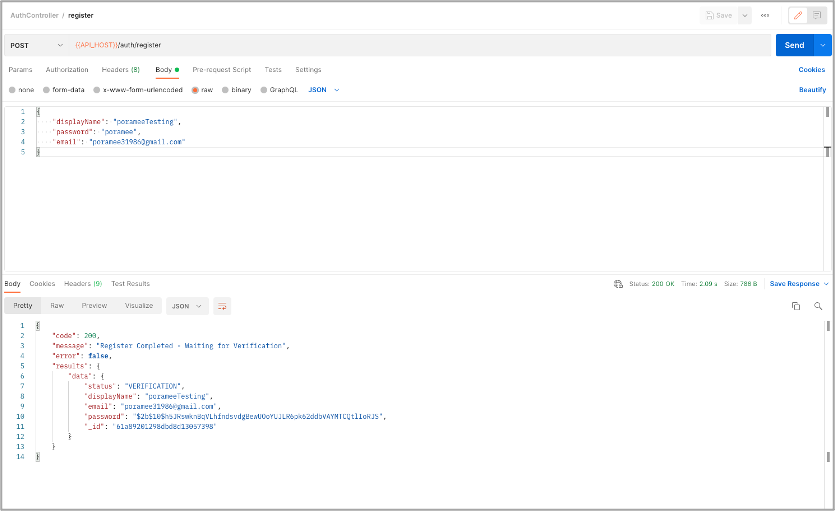
\includegraphics[width=15cm]{./chapter_4/API-register.png}
	\caption{แสดงผลการทดลอง API ของการลงทะเบียนเข้าใช้งาน}
\end{figure}
\begin{figure}
	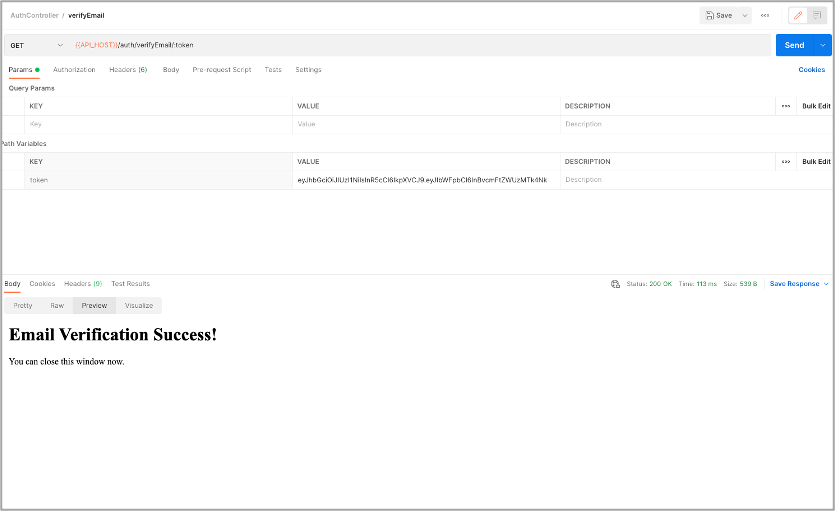
\includegraphics[width=15cm]{./chapter_4/API-token.png}
	\caption{แสดงผลการทดลอง API ของการยืนยันอีเมลด้วย Token}
\end{figure}
\begin{figure}
	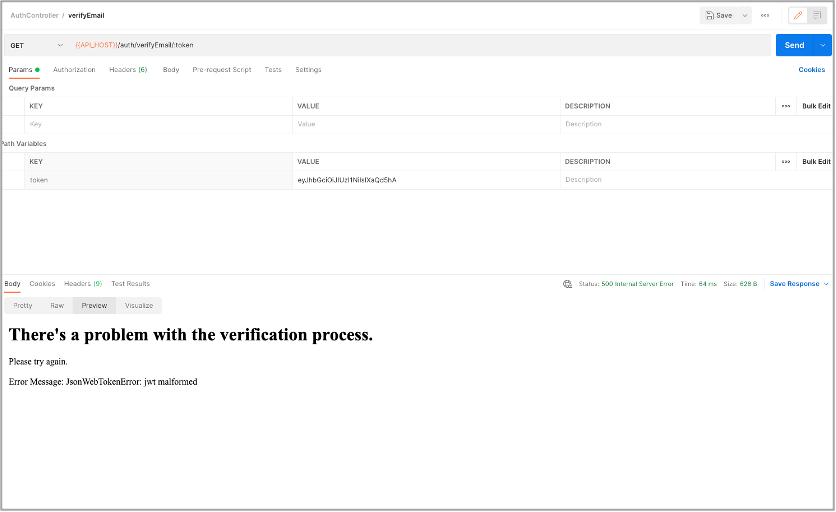
\includegraphics[width=15cm]{./chapter_4/API-token-wrong.png}
	\caption{แสดงผลการทดลอง API ของการยืนยันอีเมลด้วย Token ในกรณีที่ Token ไม่ถูกต้อง}
\end{figure}














